\documentclass[english]{article}
%    qcircuit version 2.6.0
%    Contributors: Steve Flammia, Bryan Eastin, Travis Scholten
%    This program is free software; you can redistribute it and/or modify
%    it under the terms of the GNU General Public License as published by
%    the Free Software Foundation; either version 2 of the License, or
%    (at your option) any later version.
%
%    This program is distributed in the hope that it will be useful,
%    but WITHOUT ANY WARRANTY; without even the implied warranty of
%    MERCHANTABILITY or FITNESS FOR A PARTICULAR PURPOSE.  See the
%    GNU General Public License for more details.
%
%    You should have received a copy of the GNU General Public License
%    along with this program; if not, write to the Free Software
%    Foundation, Inc., 59 Temple Place, Suite 330, Boston, MA  02111-1307  USA

% Thanks to the Xy-pic guys, Kristoffer H Rose, Ross Moore, and Daniel Müllner,
% for their help in making Qcircuit work with Xy-pic version 3.8.  
% Thanks also to Dave Clader, Andrew Childs, Rafael Possignolo, Tyson Williams,
% Sergio Boixo, Cris Moore, Jonas Anderson, and Stephan Mertens for helping us test 
% and/or develop the new version.
\ProvidesPackage{qcircuit}[2018/08/14]
\RequirePackage{xy}

\DeclareOption{braket}{
    \newcommand{\bra}[1]{\ensuremath{\left\langle{#1}\right\vert}}
    \newcommand{\ket}[1]{\ensuremath{\left\vert{#1}\right\rangle}}
    }

\DeclareOption{qm}{
    \newcommand{\ip}[2]{\ensuremath{\left\langle{#1}\middle\vert{#2}\right\rangle}}
    \newcommand{\melem}[3]{\ensuremath{\left\langle{#1}\middle\vert{#2}\middle\vert{#3}\right\rangle}}
    \newcommand{\expval}[1]{\ensuremath{\left\langle #1 \right\rangle}}
    \newcommand{\op}[2]{\ensuremath{\left\vert{#1}\middle\rangle\middle\langle{#2}\right\vert}}
}

\ProcessOptions\relax

\xyoption{matrix}
\xyoption{frame}
\xyoption{arrow}
\xyoption{arc}

\usepackage{ifpdf}
\ifpdf
\else
\PackageWarningNoLine{Qcircuit}{qcircuit is not loading in PDF mode. Activating all Xy-pic features to compensate. If you wish to use specific drivers for Xy-pic, you must modify the code in qcircuit.sty}
%    The following option loads all the features in Xy-pic. This
%    this is included as work-around to ensure documents compile
%    images correctly when using XeLaTeX.
\xyoption{all}
\fi

% The following resets Xy-pic matrix alignment to the pre-3.8 default, as
% required by Qcircuit.
\entrymodifiers={!C\entrybox}

\newcommand{\qw}[1][-1]{\ar @{-} [0,#1]}
    % Defines a wire that connects horizontally.  By default it connects to the object on the left of the current object.
    % WARNING: Wire commands must appear after the gate in any given entry.
\newcommand{\qwx}[1][-1]{\ar @{-} [#1,0]}
    % Defines a wire that connects vertically.  By default it connects to the object above the current object.
    % WARNING: Wire commands must appear after the gate in any given entry.
\newcommand{\qwa}[1][-1]{\ar @{<-} [0,#1]}
    % Defines a wire that connects horizontally with an arrow.  By default it makes an end wire with an arrow indicating the end of the circuit.
    % WARNING: Wire commands must appear after the gate in any given entry.
\newcommand{\cw}[1][-1]{\ar @{=} [0,#1]}
    % Defines a classical wire that connects horizontally.  By default it connects to the object on the left of the current object.
    % WARNING: Wire commands must appear after the gate in any given entry.
\newcommand{\cwx}[1][-1]{\ar @{=} [#1,0]}
    % Defines a classical wire that connects vertically.  By default it connects to the object above the current object.
    % WARNING: Wire commands must appear after the gate in any given entry.
\newcommand{\cwa}[1][-1]{\ar @{<=} [0,#1]}
    % Defines a classical wire that connects horizontally with an arrow.  By default it makes an end wire with an arrow indicating the end of the circuit.
    % WARNING: Wire commands must appear after the gate in any given entry.
\newcommand{\cds}[2]{*+<1em,.9em>{\hphantom{#2}} \POS [0,0].[#1,0]="e",!C *{#2};"e"+ R \qw}
    % Allows the insertion of text without a box and exands circuit around this text.
    % This is useful for such things as ... to indicate a generalized circuit.
\newcommand{\barrier}[2][-0.95em]{\ar @{--}[#2,1]+<#1, -1em>;[0,1]+<#1, 1em>}
    % Defines a barrier that is represented by a horizontal dashed line.
    % It takes a a single argument to specify how many bits to cover
    % To center the barrier between gates you can adjust the horizontal offset
    % with an optional second parameter. This is the horizontal offset in em.
    % It defaults to -0.95em
    % WARNING: Be sure to place the barrier on the topmost bit it covers, it only propogates downwards
\newcommand{\gate}[1]{*+<.6em>{#1} \POS ="i","i"+UR;"i"+UL **\dir{-};"i"+DL **\dir{-};"i"+DR **\dir{-};"i"+UR **\dir{-},"i" \qw}
    % Boxes the argument, making a gate.
\newcommand{\sgate}[2]{\gate{#1}  \qwx[#2]}
    % Creates a gate and a qwx wire going #2 spots below, for a gate split over
    % non-adjacent rows
\newcommand{\meter}{*=<1.8em,1.4em>{\xy ="j","j"-<.778em,.322em>;{"j"+<.778em,-.322em> \ellipse ur,_{}},"j"-<0em,.4em>;p+<.5em,.9em> **\dir{-},"j"+<2.2em,2.2em>*{},"j"-<2.2em,2.2em>*{} \endxy} \POS ="i","i"+UR;"i"+UL **\dir{-};"i"+DL **\dir{-};"i"+DR **\dir{-};"i"+UR **\dir{-},"i" \qw}
    % Inserts a measurement meter.
    % In case you're wondering, the constants .778em and .322em specify
    % one quarter of a circle with radius 1.1em.
    % The points added at + and - <2.2em,2.2em> are there to strech the
    % canvas, ensuring that the size is unaffected by erratic spacing issues
    % with the arc.
\newcommand{\metersymb}{\xy ="j","j"-<.778em,.322em>;{"j"+<.778em,-.322em> \ellipse ur,_{}},"j"-<0em,.4em>;p+<.5em,.9em> **\dir{-},"j"+<2.2em,2.2em>*{},"j"-<2.2em,2.2em>*{} \endxy}
    % A longer meter
\newcommand{\meterB}[1]{*=<1.8em,2.6em>{\xy 0;<0em,-.8em>:
0*{\begingroup
\everymath{\scriptstyle}
\tiny #1 \endgroup},<0em,.7em>*{\xy ="j","j"-<.778em,-.322em>;{"j"+<.778em,.322em> \ellipse ur,_{}},"j"-<0em,-.2em>;p+<.5em,.9em> **\dir{-},"j"+<2.2em,2.2em>*{},"j"-<2.2em,2.2em>*{} \endxy} 
\endxy} \POS ="i","i"+UR;"i"+UL **\dir{-};"i"+DL **\dir{-};"i"+DR **\dir{-};"i"+UR **\dir{-},"i" \qw}
    % A meter that allows for a measurement operator to be added below
\newcommand{\smeterB}[2]{\meterB{#1} \qwx[#2] \qw}
    % A split meter that allows for a measurement operator to be split over non-
    % adjacent rows
\newcommand{\measure}[1]{*+[F-:<.9em>]{#1} \qw}
    % Inserts a measurement bubble with user defined text.
\newcommand{\measuretab}[1]{*{\xy*+<.6em>{#1}="e";"e"+UL;"e"+UR **\dir{-};"e"+DR **\dir{-};"e"+DL **\dir{-};"e"+LC-<.5em,0em> **\dir{-};"e"+UL **\dir{-} \endxy} \qw}
    % Inserts a measurement tab with user defined text.
\newcommand{\measureD}[1]{*{\xy*+=<0em,.1em>{#1}="e";"e"+UR+<0em,.25em>;"e"+UL+<-.5em,.25em> **\dir{-};"e"+DL+<-.5em,-.25em> **\dir{-};"e"+DR+<0em,-.25em> **\dir{-};{"e"+UR+<0em,.25em>\ellipse^{}};"e"+C:,+(0,1)*{} \endxy} \qw}
    % Inserts a D-shaped measurement gate with user defined text.
\newcommand{\multimeasure}[2]{*+<1em,.9em>{\hphantom{#2}} \qw \POS[0,0].[#1,0];p !C *{#2},p \drop\frm<.9em>{-}}
    % Draws a multiple qubit measurement bubble starting at the current position and spanning #1 additional gates below.
    % #2 gives the label for the gate.
    % You must use an argument of the same width as #2 in \ghost for the wires to connect properly on the lower lines.
\newcommand{\multimeasureD}[2]{*+<1em,.9em>{\hphantom{#2}} \POS [0,0]="i",[0,0].[#1,0]="e",!C *{#2},"e"+UR-<.8em,0em>;"e"+UL **\dir{-};"e"+DL **\dir{-};"e"+DR+<-.8em,0em> **\dir{-};{"e"+DR+<0em,.8em>\ellipse^{}};"e"+UR+<0em,-.8em> **\dir{-};{"e"+UR-<.8em,0em>\ellipse^{}},"i" \qw}
    % Draws a multiple qubit D-shaped measurement gate starting at the current position and spanning #1 additional gates below.
    % #2 gives the label for the gate.
    % You must use an argument of the same width as #2 in \ghost for the wires to connect properly on the lower lines.
\newcommand{\control}{*!<0em,.025em>-=-<.2em>{\bullet}}
    % Inserts an unconnected control.
\newcommand{\controlo}{*+<.01em>{\xy -<.095em>*\xycircle<.19em>{} \endxy}}
    % Inserts a unconnected control-on-0.
\newcommand{\ctrl}[1]{\control \qwx[#1] \qw}
    % Inserts a control and connects it to the object #1 wires below.
\newcommand{\ctrlo}[1]{\controlo \qwx[#1] \qw}
    % Inserts a control-on-0 and connects it to the object #1 wires below.
\newcommand{\cctrl}[1]{\control \cwx[#1] \cw}
    % Inserts a classical control and connects it to the object #1 wires below. 
\newcommand{\cctrlo}[1]{\controlo \cwx[#1] \cw}
    % Inserts a classical control-on-0 and connects it to the object #1 wires below.    
\newcommand{\targ}{*+<.02em,.02em>{\xy ="i","i"-<.39em,0em>;"i"+<.39em,0em> **\dir{-}, "i"-<0em,.39em>;"i"+<0em,.39em> **\dir{-},"i"*\xycircle<.4em>{} \endxy} \qw}
    % Inserts a CNOT target.
\newcommand{\qswap}{*=<0em>{\times} \qw}
    % Inserts half a swap gate.
    % Must be connected to the other swap with \qwx.
\newcommand{\multigate}[2]{*+<1em,.9em>{\hphantom{#2}} \POS [0,0]="i",[0,0].[#1,0]="e",!C *{#2},"e"+UR;"e"+UL **\dir{-};"e"+DL **\dir{-};"e"+DR **\dir{-};"e"+UR **\dir{-},"i" \qw}
    % Draws a multiple qubit gate starting at the current position and spanning #1 additional gates below.
    % #2 gives the label for the gate.
    % You must use an argument of the same width as #2 in \ghost for the wires to connect properly on the lower lines.
\newcommand{\ghost}[1]{*+<1em,.9em>{\hphantom{#1}} \qw}
    % Leaves space for \multigate on wires other than the one on which \multigate appears.  Without this command wires will cross your gate.
    % #1 should match the second argument in the corresponding \multigate.
\newcommand{\cghost}[1]{*+<1em,.9em>{\hphantom{#1}} \cw}
    % Same as ghost but with a classical incoming wire.
\newcommand{\nghost}[1]{*+<1em,.9em>{\hphantom{#1}}}
    % Same as ghost but with no incoming wire.
\newcommand{\push}[1]{*{#1}}
    % Inserts #1, overriding the default that causes entries to have zero size.  This command takes the place of a gate.
    % Like a gate, it must precede any wire commands.
    % \push is useful for forcing columns apart.
    % NOTE: It might be useful to know that a gate is about 1.3 times the height of its contents.  I.e. \gate{M} is 1.3em tall.
    % WARNING: \push must appear before any wire commands and may not appear in an entry with a gate or label.
\newcommand{\gategroup}[6]{\POS"#1,#2"."#3,#2"."#1,#4"."#3,#4"!C*+<#5>\frm{#6}}
    % Constructs a box or bracket enclosing the square block spanning rows #1-#3 and columns=#2-#4.
    % The block is given a margin #5/2, so #5 should be a valid length.
    % #6 can take the following arguments -- or . or _\} or ^\} or \{ or \} or _) or ^) or ( or ) where the first two options yield dashed and
    % dotted boxes respectively, and the last eight options yield bottom, top, left, and right braces of the curly or normal variety.  See the Xy-pic reference manual for more options.
    % \gategroup can appear at the end of any gate entry, but it's good form to pick either the last entry or one of the corner gates.
    % BUG: \gategroup uses the four corner gates to determine the size of the bounding box.  Other gates may stick out of that box.  See \prop.
\newcommand{\inputgroupv}[5]{\POS"#1,1"."#2,1"."#1,1"."#2,1"!C*+<#3>\frm{\{}, \POS"#1,1"."#2,1"."#1,1"."#2,1"*!C!<1.7em,#4>=<0em>{#5}}
    % Constructs an input group with label #5 and a grouping { from rows #1 to #2 with #3 and #4 controlling the spacing
\newcommand{\inputgroup}[4]{\POS"#1,1"."#2,1"."#1,1"."#2,1", \POS"#1,1"."#2,1"."#1,1"."#2,1"*!C!<1em,#3>=<0em>{#4}}
    % Constructs an input group with label #4 from rows #1 to #2 with #3 controlling the spacing
\newcommand{\inputgrouph}[5]{\POS"#1,1"."#2,1"."#1,1"."#2,1", \POS"#1,1"."#2,1"."#1,1"."#2,1"*!C!<#5,#3>=<0em>{#4}}
    % Constructs an input group with label #4 and a grouping /vdots from rows #1 to #2 with #3 and #5 controlling the spacing
\newcommand{\rstick}[1]{*!L!<-.5em,0em>=<0em>{#1}}
    % Centers the left side of #1 in the cell.  Intended for lining up wire labels.  Note that non-gates have default size zero.
\newcommand{\lstick}[1]{*!R!<.5em,0em>=<0em>{#1}}
    % Centers the right side of #1 in the cell.  Intended for lining up wire labels.  Note that non-gates have default size zero.
\newcommand{\ustick}[1]{*!D!<0em,-.5em>=<0em>{#1}}
    % Centers the bottom of #1 in the cell.  Intended for lining up wire labels.  Note that non-gates have default size zero.
\newcommand{\dstick}[1]{*!U!<0em,.5em>=<0em>{#1}}
    % Centers the top of #1 in the cell.  Intended for lining up wire labels.  Note that non-gates have default size zero.
\newcommand{\Qcircuit}{\xymatrix @*=<0em>}
    % Defines \Qcircuit as an \xymatrix with entries of default size 0em.
\newcommand{\link}[2]{\ar @{-} [#1,#2]}
    % Draws a wire or connecting line to the element #1 rows down and #2 columns forward.
\newcommand{\pureghost}[1]{*+<1em,.9em>{\hphantom{#1}}}
    % Same as \ghost except it omits the wire leading to the left. 

\endinput



% packages
\usepackage[T1]{fontenc}
\usepackage[utf8]{inputenc}
\usepackage{graphicx}
\usepackage{hyperref}
\usepackage{amssymb}
\usepackage{amsmath}
\usepackage[toc,page]{appendix}
\usepackage{listings}
\usepackage{enumitem}
\usepackage{tikz}
\usepackage{braket}

% commands
\newcommand{\sbigotimes}{%
	\mathop{\mathchoice{\textstyle\bigotimes}{\bigotimes}{\bigotimes}{\bigotimes}}%
}
\newcommand{\zeroket}{\begin{pmatrix} 1 \\ 0 \end{pmatrix}}
\newcommand{\oneket}{\begin{pmatrix} 0 \\ 1 \end{pmatrix}}

\graphicspath{{img/}}

\begin{document}
	\title{An Introduction to Quantum Computing for Computer Scientists, with SAT}
	\author{Francesco Piro}
	\maketitle
	
	\begin{abstract}
		This is the paper I have produced during my study of quantum computing for solving the SAT problem...
	\end{abstract}

	% definire meglio la struttura ci sono:
	% definizioni
	% esempi
	% riferimenti al codice nell appendice
	% important conclusions
	
	\section*{Introduction}
	\label{sec:introduction}
	Quantum computation is a wide area involving several disciplines that is having always more success in nowadays applications thanks in particular to the development of the technology and its incredible results. Quantum physics' principles are the fundamentals on which the entire theory is based: thanks to their properties, new architectures allow to define devices that can solve classical problems in surprisingly reduced time and space complexities. However we always have a trade-off to consider, in particular now that these technology are still emerging.\\
	
	This paper aims at giving a description for computer scientists of what a quantum computer is and which are its real impacts and advantages with respect to the classical ones. Hence I will try to provide a description of the state of the art of quantum computing with an approach that allows to understand how from the basic principles of quantum mechanics we are able to have an algorithm that is faster with respect to its classic counterpart. In order to do so in the first chapter (\ref{sec:quantumComputing}) I will start with the basic linear algebra needed to study the quantum physics' principles we need to define a quantum computer. The definition of the \emph{quantum computer} is fundamental both to understand how and algorithm is executed but also to have a comparison with the classic Turing machine that allows us to determine conclusions on computational complexity (chapter \ref{sec:computationalTheory}). In the first chapter we will also have practical examples realized with the \textbf{qiskit library} in order to clarify also with some lines of code the concepts. Once the background on quantum computation and computational theory are well consolidated by the reader, the last chapters provide a practical example that is used to prove the speedup for the particular \textbf{satisfiability problem.} I have used an efficient classical solver for the \emph{k-SAT} as I could compare it with my quantum implementation, both realized in python. In the end I provide some important conclusions for quantum computing that I was able to conclude thanks to my study, in particular in the papers listed in the references.
	
	\section{Quantum Computing}
	\label{sec:quantumComputing}
		This chapter aims at providing first the fundamentals needed in order to deal with quantum mechanics and second at defining a quantum computer thanks to the principles previously identified. With the quantum device we will be able to make a comparison with the classical one to understand with examples how the basic operations are realized in order to use them to implement complete algorithms. Further in the chapter, a section is completely dedicated to the main quantum search algorithm that is fundamental to solve the SAT with a quantum algorithm. Also here we will start from a classical version to compare it with its quantum counterpart. All the arguments related in this chapter, together with the ones in the next (\ref{sec:computationalTheory}) are fundamental to give a significant interpretation to the comparison between the classic and quantum implementation of the algorithm able to solve the \textbf{satisfiability problem} (\ref{sec:sat}).
		
		\subsection{Fundamentals}
		\label{sec:fundamentals}
			The study of quantum computers requires the knowledge of the decimal and binary representation of integers, probability notions and in particular linear algebra fundamental definitions like the ones of: \emph{vectors, spaces, bases, linear systems, tensor product...}. In this section are presented the basic concepts needed to face the quantum physics principles that we need in order to realize our quantum computer. 
			
			\subsubsection{Linear Algebra}
			\label{sec:linearAlgebra}
			Basic principles of linear algebra are assumed to be well known by the reader, I want now to remark only the most important operators and definitions that we need to face the definition of the following quantum mechanical theorems we need to define a quantum device. The most important notions we need to acquire from this section are: \emph{tensor product, Hilbert space, bra-ket notation}.\\
			
			In order to realize a quantum computer we need understand how to define a state that is able to contain information that can be used to obtain a certain objective. As we will see in the next section, the state of a quantum device is a quantum state, thus a mathematical model that lives into a specific \emph{vector state} whose dimension depends on the amount of information it needs to take care of. Typically, significant states contain information that results from the composition of several spaces combined together thanks to a particular operator called tensor product.
			
			\paragraph{Definition (Tensor Product):} \emph{Given two vector spaces V and W over a field K with bases $e_1,..., e_m$ and
$f_1,..., f_n$ respectively, the tensor product $V \otimes W$ is another vector space over K of dimension
mn. The tensor product space is equipped with a bilinear operation $\otimes : V \times W \rightarrow V \otimes W$. The
vector space $V \otimes W$ has basis $e_i \otimes f_j \forall i = 1,...,m, j = 1,...,n$}. \\
			
			Typically we are going to work with complex Euclidean vector spaces of the form $\mathbb{C}^n$ and, by choosing the standard basis in the origin vector spaces, then the tensor product is nothing more than the Kronecker product.
			
			\paragraph{Definition (Kronecker Product):} \emph{Given $A \in \mathbb{C}^{m\times n}$, $B \in \mathbb{C}^{p\times q}$, the Kronecker product $A \otimes B$ is the matrix $D \in \mathbb{C}^{mp\times nq}$ defined as:}
			\begin{center}
				$
				D = A\otimes B =
				\begin{pmatrix}
				a_{11}B & \cdots & a_{1n}B \\
				a_{21}B & \cdots  & a_{2n}B \\
				\vdots & \vdots & \vdots \\
				a_{m1}B & \cdots & a_{mn}B
				\end{pmatrix}
				$
			\end{center}
		
			Now that we know the notions of vector state and Tensor product, we can use them to define an important space (in particular for the SAT problem we are going to study later) called the \textbf{Hilbert space} and denoted with $\mathcal{H}$.
			
			\paragraph{Definition (Hilbert Space):} \emph{Given the complex space $\mathbb{C}$ we define the Hilbert space $\mathcal{H}$ as the (n + 1)-tuple tensor product:}
			\begin{center}
				$
				\mathcal{H} := \sbigotimes_1^{n+1} \mathbb{C}^{2}
				$
			\end{center}
		
			As we said, in the Hilbert space we will carry the discussion of the SAT problem but to understand what the result of this tensor product actually defines we still need to give probably the most important definition. In order to represent a quantum state we use the so called \emph{bra-ket notation} introduced in 1939 by Paul Dirac.
			
			\paragraph{Definition (Dirac/bra-ket Notation):} \emph{Given a complex Euclidean space $\mathbb{S} \equiv \mathbb{C}^{n}$, $|\psi\rangle \in \mathbb{S}$ denotes a column vector, and $\langle\psi| \in \mathbb{S}^{*}$ denotes a row vector that is the conjugate transpose of $|\psi\rangle$, i.i. $\langle\psi| = |\psi\rangle$. The vector $|\psi\rangle$ is also called a ket, while the vector $\langle\psi|$ is also called a bra.} \\
			
			The bra-ket notation allows us to define a quantum state, hence a vector that lives into a particular vector space. Its definition intrinsically defines also the result of combining two states living in the same state with the \textbf{inner product}, straightforwardly obtained from what we have just said: $\langle\psi|\phi\rangle$. This result is fundamental to define spaces that are higher than one only dimension as the Hilbert state presented before. To understand what $\mathcal{H}$ is we can now use two examples where we define the basis of the first two results obtained by doing the tensor product of the complex space $\mathbb{C}^{2}$ with itself. Remember that the basis of a space is the smallest set of linearly independent vectors that can be used to represents all the vectors that belong to that space.
			
			\paragraph{Example 1:} 
			\label{ex:c2}
			\emph{Considering the basic case of $\mathbb{C}^{2}$ the basis can be trivially identified as:}
			\begin{center}
				$|0\rangle = \zeroket \hspace{1cm} |1\rangle = \begin{pmatrix} 0 \\ 1 \end{pmatrix}$
			\end{center}
		
			\paragraph{Example 2:} 
			\label{ex:c4}
			\emph{Considering a single product, thus $\sbigotimes_1^{1} \mathbb{C}^{2} = \mathbb{C}^{2} \otimes \mathbb{C}^{2}$, we obtain the basis by multiplying in all possible ways the vectors of the basis of the previous example. We now have kets of dimension 2, thus vectors with 4 lines and 1 column:}
			\begin{center}
					$
					|00\rangle = |0\rangle \otimes |0\rangle = \zeroket \otimes \zeroket = 
					\begin{pmatrix}
					1\zeroket \vspace{3pt} \\
					0\zeroket
					\end{pmatrix} =
					\begin{pmatrix}
					1 \\ 0 \\ 0 \\ 0
					\end{pmatrix}
					$\vfill
					$
					|01\rangle = |0\rangle \otimes |1\rangle = \zeroket \otimes \oneket = 
					\begin{pmatrix}
					1\oneket \vspace{3pt} \\
					0\oneket
					\end{pmatrix} =
					\begin{pmatrix}
					0 \\ 1 \\ 0 \\ 0
					\end{pmatrix}
					$ \vfill
					$
					|10\rangle = |1\rangle \otimes |0\rangle = \oneket \otimes \zeroket = 
					\begin{pmatrix}
					0\zeroket \vspace{3pt} \\
					1\zeroket
					\end{pmatrix} =
					\begin{pmatrix}
					0 \\ 0 \\ 1 \\ 0
					\end{pmatrix}
					$ \vfill
					$
					|11\rangle = |1\rangle \otimes |1\rangle = \oneket \otimes \oneket = 
					\begin{pmatrix}
					0\oneket \vspace{3pt} \\
					1\oneket
					\end{pmatrix} =
					\begin{pmatrix}
					0 \\ 0 \\ 0 \\ 1
					\end{pmatrix}
					$
			\end{center}
		
			Thanks to these two examples we can generalize to the n + 1 case and obtain the definition of the Hilbert space we gave before. \\
			
			Before starting with the quantum physics section where we will start by defining the smallest unit element we use to represent information, the so called \textbf{qubit}, we need to give one further definition. In order to perform operations on qubits we will consider (section \ref{sec:operationsOnQubits}) only a particular family of matrices called unitary matrices. These matrices allow to perform operations on qubits without modifying the basic properties of the quantum state and are defined as follows.
			
			\paragraph{Definition (Unitary Matrix):} \emph{A complex square matrix $\mathcal{U}$ is unitary if $U^{*}U = UU^{*} = I$.} \\
			
			Unitary matrices have significant importance in quantum mechanics because they are \textbf{norm-preserving}, this will be fundamental to identify the two main features of quantum operations that can now be introduced as: \emph{apply a unitary matrix on a quantum state, thus a vector whose norm will be preserved}.
						
			\subsubsection{Quantum Physics}
			\label{sec:quantumMechanics}
				Quantum mechanics is a fundamental theory in physics describing the properties of nature. We do not need entirely its entire power for our purpose but, starting from some basic concepts we will exploit some conclusions that are useful to design an algorithm that is faster than its classical counterpart. As we do when we start studying computer science, we want to identify the smallest, most basic element that allows us to represent the information. From a classical point of view we have the \textbf{bit} whose values can be either 1 or 0. From a quantum point of view, instead, we have the \textbf{qubit}, complex variables that can assume values ranging from 0 to 1 (in modulus), identified in a complex space over a surface called the \emph{Block Sphere}.
				
				\paragraph{Definition (Qubit:)} \emph{The qubit is the smallest unit of measurement used to quantify information in quantum computing. It identifies the bit in a superposition, hence both 0 and 1 values are considered. Formally it is a vector of the space $\mathbb{C}^{2}$ represented as a linear combination of the elements contained in its basis (\ref{ex:c2}). A qubit $\psi$, with $\alpha_0,\alpha_1\in\mathbb{C}$, is defined as:}\\
				\begin{center}
					$
					|\psi\rangle = \alpha_0 |0\rangle + \alpha_1 |1\rangle = \alpha_0\zeroket + \alpha_1\oneket
					$
				\end{center}
				
				To understand better the definition of the qubit we now provide its representation in a tridimensional space whose directions are obtained from basic linear algebra principles that are not now relevant. We now just need to understand that, thanks to the coefficients $\alpha_0$ and $\alpha_1$ belonging to the complex space $\mathbb{C}$ we are able to consider the basic element of our computation as one of the infinite points that live over the surface of a sphere. We can grasp in this concept a first hint in the advantages that quantum states provide with respect their classic counterpart.
				
				\paragraph{Definition (Block Sphere):} \emph{The Block Sphere is the geometrical representation of the pure state space of a two-level quantum mechanical system. In other words it represents all the possible vectors that can be obtained by combining the vectors of the basis for a quantum register of 1 qubit.}\\
				
				Consider the following examples to understand how vectors are represented in the Bloch sphere; we present the trivial cases for both $|0\rangle$ and $|1\rangle$ and the respective orthogonal vectors identifying the x and y axes.
	
				\paragraph{Example 3:} \emph{Consider the qubit $\psi$, with $\alpha_0,\alpha_1\in\mathbb{C}$, such that: 	$|\psi\rangle = \alpha_0 |0\rangle + \alpha_1 |1\rangle$. (Check code at \ref{c:example3})}
				
				\begin{enumerate}
					\centering
					\begin{figure}[h]
						\begin{minipage}{0.4\textwidth}
							\item $\alpha_0=1, \;\alpha_1=0$
							\centering
							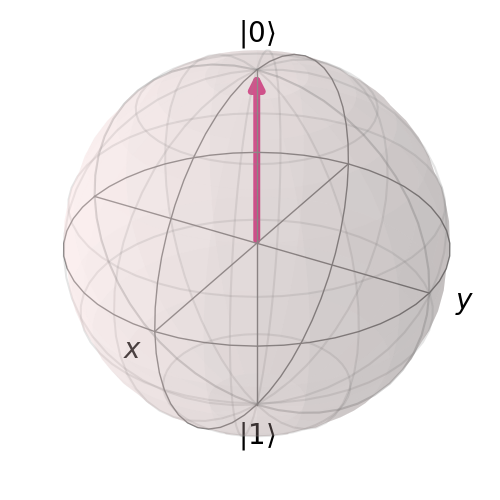
\includegraphics[scale=0.4]{zeroket.png}
							\caption{$|\psi\rangle= |0\rangle$}
						\end{minipage} \hfill
						\begin{minipage}{0.4\textwidth}
							\item $\alpha_0=0, \;\alpha_1=1$
							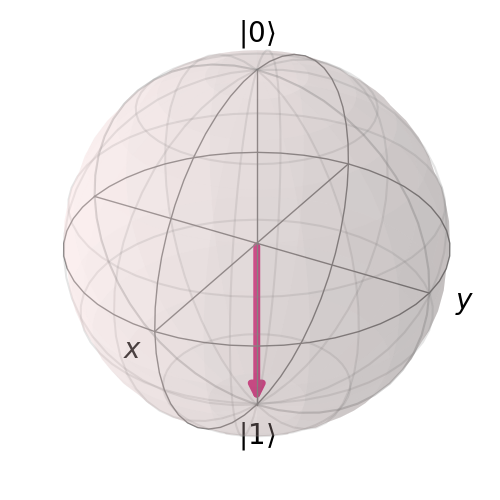
\includegraphics[scale=0.4]{oneket.png}
							\caption{$|\psi\rangle= |1\rangle$}
						\end{minipage}
					\end{figure}
					\begin{figure}[h]
						\begin{minipage}{0.4\textwidth}
							\item $\alpha_0=\frac{1}{\sqrt{2}}, \;\alpha_1=\frac{1}{\sqrt{2}}$
							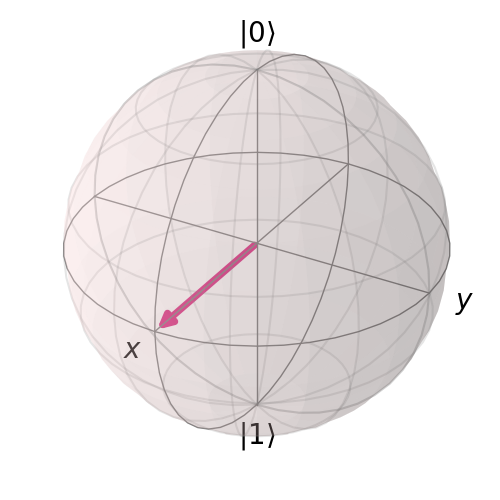
\includegraphics[scale=0.4]{xket.png}
							\caption{$|\psi\rangle = \frac{1}{\sqrt{2}}(|0\rangle+|1\rangle)$}
						\end{minipage} \hfill
						\begin{minipage}{0.4\textwidth}
							\item $\alpha_0=\frac{1}{\sqrt{2}}, \;\alpha_1=\frac{i}{\sqrt{2}}$
							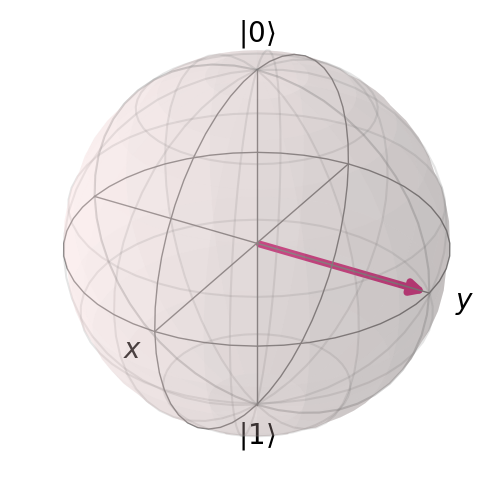
\includegraphics[scale=0.4]{yket.png}
							\caption{$|\psi\rangle = \frac{1}{\sqrt{2}}(|0\rangle+i|1\rangle)$}
						\end{minipage}
					\end{figure}
				\end{enumerate}
			
			Obviously we can also represent vectors that belong to spaces with a higher dimension than 2, in this case we will have their representation over a hypersphere (check the plot\_bloch\_multivector method in the qiskit library). As in classical computer we haver registers, defined as a sequence of bits, in quantum computing we have \emph{quantum-registers} composed of a sequence of qubits. Typically a quantum computer has a single quantum-register made up of qubits (see section \ref{sec:quantumComputer}). It is now important to remark the first important conclusion on quantum computing, that derives from the definition of quantum-register that we have just provided. We see that $\sbigotimes_1^{n+1} \mathbb{C}^{2}$ is a $2^{n}$ dimensional space. This is sharp in contrast with what happens for classical registers: given n classical bits, their state is a binary string in $\{0,1\}^{n}$, thus an n-dimensional space. In other words we arrive to the first important conclusion.
			
			\paragraph{Conclusion 1:} \emph{the dimension of the state space of quantum registers grows exponentially in the number of qubits, whereas the dimension of the state space of classical registers grows linearly in the number of bits.}
			
			\subsubsection{Superposition}
			\label{sec:superposition}
				The mathematical definition of the qubit we have just seen is useful to understand the first difference between the representation of a state either in classical or quantum fields. We want now to define from a more physical point of view what means for a qubit to assume both the value 0 and 1. The basic physical principle behind this property is the \emph{Heisenberg indetermination principle}, but without going too deep in the details let's try to understand it with a simple example. 
				
				\paragraph{Example 4:} \emph{We have seen that bits can assume at a certain time instant one and one value only. Considering now a qubit we could say that it assumed both the values 1 and 0 because its definition is based on Heisenberg's principle, basically stating that particles can assume at the same time different positions. This is a physics principle: electrons can be at the same time in different positions. That is why considering the position 0 and the position 1 we can say that a qubit is situated in both of them. The sad reality is that we do not know the real state of the qubit until we perform a specific operation on it, called measurement, which makes it collapse either to a 0 or a 1 "boring" bit. The following picture tries to illustrate the principle of an electron whose real position is not deterministic until this operation.}
				
				\begin{figure}[h]
					\centering
					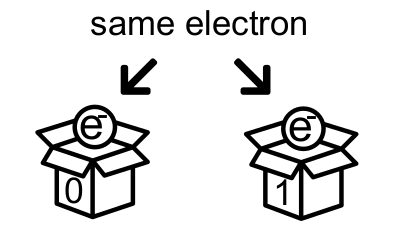
\includegraphics[scale=0.75]{superposition.png}
					\caption{Superposition of the electron}
				\end{figure}
			
				As we may have understood superposition is a very interesting property, also because it can be generalized to the case of n qubits rather than just one. We will se in the implementation of the SAT algorithm how operations on multiple qubits are able to exploit superposition in order to compute the solution of the problem. With this property we can start guessing how algorithms will be run on our quantum computer: from a certain initial state we will perform operations that exploit the indetermination principle over the qubits, thus considering several states at the same time, until the end when performing the measurement we will make them collapse to a single string of 1s and 0s which is our result.
			
			\subsubsection{Entanglement}
			\label{sec:entanglement}
				Entanglement is the second main feature of quantum computers that, together with superposition, differentiates them from quantum computers. These are in fact the two main features that are exploited in algorithms to find the solution of a problem. \\
				
				To understand entanglement we start by answering the following question: \\ \\				
				$\underline{What \; do \; we \; gain \; by \; moving \; from \; single \; qubits \; spaces \; to \; multiple \; qubits \; spaces?}$ \\
				
				The answer has two motivations, the first regarding the states representation the second the property of entanglement:
				\begin{enumerate}[label=(\roman*)]
					\item As we described before, also in quantum computing we will need to define registers that contain more than 1 qubit. To do so it suffices to compose a vector of n qubits which identify the state obtained by the result of their quantum product.
					
					\item Linear algebra definitions, in particular for what concerns the tensor products, show that not every state that we consider can be represented as the tensor product of n-qubits. Whenever we have to deal with a state of that kind we will say that the quantum state is entangled.
				\end{enumerate}
			
				More formally the definition of entanglement is the following:
				
				\paragraph{Definition (Entanglement):} \emph{A quantum state $|\psi\rangle \in \sbigotimes_1^{n+1} \mathbb{C}^{2}$ is a product state if it can be expressed as a tensor product $|\psi_0\rangle \otimes |\psi_1\rangle \otimes \cdots \otimes |\psi_n\rangle$ of n 1-qubit states. Otherwise, it is entangled.} \\
				
				To understand better the definition let's consider the simplest example possible: considering a state living in the $\mathbb{C}^4$ complex space we want to check if it is a product state or entangled by looking for two 1-qubit states whose tensor product is the state that we are dealing with. We will see next how the entanglement feature can be used, in particular what still happens when 2 qubits are entangled together.
				
				\paragraph{Example 5:} \emph{Consider the following 2-qubit state:
				\begin{align*}
					\frac{1}{2}|00\rangle+\frac{1}{2}|01\rangle+\frac{1}{2}|10\rangle+\frac{1}{2}|11\rangle
				\end{align*} 
				This is a product state because we can find two states whose tensor product is the starting one: $\frac{1}{2}(|0\rangle+|1\rangle)\otimes\frac{1}{2}(|0\rangle+|1\rangle)$. By contrast, the 2-qubit state:
				\begin{align*}
					\frac{1}{\sqrt{2}}|00\rangle+\frac{1}{\sqrt{2}}|11\rangle
				\end{align*}
				is an entangled state, because it can not be expressed as the tensor product of two 1-qubit states.} \\
			
				The actual meaning of entanglement can be fully appreciated only once we have defined the measurement, but we can start grasping its importance thanks to the algebraic definition that we have just provided. Having an entangled state means that we can not find two qubits whose tensor product result is the one that we are considering, this because there are not two "linearly independent" states satisfying such property. In conclusion the qubits that compose an entangled state are in some way related one with the other, in other words: \emph{when two or more qubits are entangled, they affect each other, and measuring one qubit changes the probability distribution for the other qubits.}
				
			\subsubsection{Operations on Qubits}
			\label{sec:operationsOnQubits}
				The definition of qubit should be clear now, moreover we have also understood that a quantum computer is composed of a quantum register where multiple qubits are used in order to move from a state to another. We want now to understand how to perform operations on qubits (without breaking the basic properties of the quantum state) so that we can implement algorithms that allow to solve problems incrementally going through different quantum states. First of all we have to give the definition of a quantum operation on n qubits:
				
				\paragraph{Definition (Quantum Gates):} \emph{An operation performed by a quantum computer with n qubits, also called a gate, is a unitary matrix in $\mathbb{C}^{2^{n}\times2^{n}}$.} \\
				
				Thus, for an n-qubit system, the quantum state is a unit vector $|\psi\rangle\in\mathbb{C}^{2^{n}}$, while a quantum operation is a matrix $U\in\mathbb{C}^{2^{n}\times2^{n}}$, and the application of U onto the state $|\psi\rangle$ is the unit vector $U|\psi\rangle\in\mathbb{C}^{2^{n}}$. This leads to the following important features of quantum gates:
				\begin{itemize}
					\item Quantum operations are \textbf{linear}
					\item Quantum operations are \textbf{reversible}
				\end{itemize}
				Every significant operation on a quantum state must be represented as a unitary matrix, this may seem very restrictive but it has been proved that these two features do not remove any power to the quantum computer we want to design. We can now give the following important conclusion.
				
				\paragraph{Conclusion 2:} \emph{A universal quantum computer is Turing-complete.}\\
				
				Now that we know how quantum operations are formally defined we have to show first how they operate over a set of qubits and second which are the most important gates that we need to implement quantum algorithms. A quantum algorithm is implemented with a quantum circuit: a quantum circuit is represented by indicating which operations are performed on each qubit or group of qubits. For a quantum computer with n qubits, we represent n qubits lines and operations as blocks taking as input a set of qubits and with output the same input lines. Consider the following picture as the first trivial representation where a general unitary matrix $U$ is applied over all the qubits of the quantum computer. 
				
				\begin{figure}[h]
					\centering
					\begin{minipage}{0.6\textwidth}
						\Qcircuit @C=1em @R=.7em {
							\lstick{\ket{q_0}} & \multigate{2}{U} & \qw \\
							\lstick{\ket{q_1}} & \ghost{U} & \qw \\
							\lstick{\ket{q_2}} & \ghost{U} & \qw			
						}
					\end{minipage}
					\hspace{0.3cm}
					$\equiv$
					\hspace{1cm}
					\begin{minipage}{0.6\textwidth}
						\Qcircuit @C=1em @R=.7em {
							\lstick{\ket{q_0}} & \gate{U} & \qw \\
							\lstick{\ket{q_1}} & \gate{U} & \qw \\
							\lstick{\ket{q_2}} & \gate{U} & \qw			
						}
					\end{minipage}
					\caption{Trivial equivalence of quantum circuits}
				\end{figure}
			
				In the picture above we have used a slight abuse of notation for what concerns the multigate $U$ applied over the 3-qubit state. In mathematical terms, in fact, the equivalence holds when we consider the gate $U\otimes U\otimes U$ applied to the state composed of 3 qubits. Hence, the gate of the first circuit has to be interpreted as the unitary matrix obtained from the tensor product of 3 $U$ unitary matrices, thus living in the $\mathbb{C}^{8}$ space. \\
				
				Before going to study the fundamental gates we need to implement quantum algorithms it is very important to understand how to interpret the representation of a quantum circuit. Circuit diagrams are read from left to right, but because each gate corresponds to applying a matrix to the quantum state, the matrices corresponding to the gates should be written from right to left in the mathematical representation. In the following picture, for example, the result of the circuit is the state $BA\ket{\psi}$, obtained by first applying gate $A$ and then $B$.
				
				\begin{figure}[h]
					\centering
					\mbox{
						\Qcircuit @C=1em @R=.7em {
							& \multigate{2}{A} & \qw & \multigate{2}{B} & \qw \\
							\lstick{\ket{\psi}} & \ghost{A} & \qw & \ghost{B} & \qw & \rstick{BA\ket{\psi}} \\
							& \ghost{A} & \qw & \ghost{B} & \qw
					}}
					\caption{Quantum circuit interpretation}
				\end{figure}
			
				So far it seems that every kind of unitary gate is allowed to be used in a quantum circuit, but as we are not allowed in classical algorithms to define every kind of function also in quantum computing we will define operations as unitary gates by combining a set of nice matrices which are efficiently specifiable and implementable. The only set of nice matrices we will consider in our study (which suffices to implement the SAT algorithm) are called the \emph{Pauli Operators} and they are defined as follows.
				
				\paragraph{Definition (Pauli Operators):} \emph{The Pauli operators are four single-qubit unitary matrices $I, X, Y, Z$ forming a basis for $\mathbb{C}^{2\times2}$ such that: $XYZ=iI$. The four matrices are:}
				\begin{figure}[h]
					\begin{minipage}{0.5\textwidth}
						\centering
						$
						I = \begin{pmatrix}
								1 & 0 \\
								0 & 1
						\end{pmatrix}
						$\vspace{0.2cm}
					\end{minipage}
					\begin{minipage}{0.5\textwidth}
						\centering
						$
						X = \begin{pmatrix}
								0 & 1 \\
								1 & 0
						\end{pmatrix}
						$\vspace{0.2cm}
					\end{minipage}
					\begin{minipage}{0.5\textwidth}
						\centering
						$
						Y = \begin{pmatrix}
								0 & -i \\
								i & 0
						\end{pmatrix}
						$
					\end{minipage}
					\begin{minipage}{0.5\textwidth}
						\centering
						$
						Z = \begin{pmatrix}
								1 & 0 \\
								0 & -1
						\end{pmatrix}
						$
					\end{minipage}
				\end{figure}
			
			\emph{With the definition it can be checked trivially that all $I, X, Y, Z$ are unitary.}\\
			
			Now that we know the Pauli set we can start to give the list of the most important operators we need to implement quantum algorithms by comparing them with the respective counterpart operations in classic computation:
			
			\begin{itemize} 
				\item The $X$ gate is the equivalent to the NOT gate in classical computers. Thus we have: $X\ket{0} = \ket{1}$ and $X\ket{1} = \ket{0}$. 
				
				\item The $Z$ gate has no equivalent in classical computers because it performs a phase-flip on the target qubit. Thus we have: $Z\ket{0} = \ket{0}$ and $Z\ket{1}=-1$.
				
				\item Another single-qubit fundamental gate is the Hadamard gate $H$. $H$ is still a unitary matrix that belongs to the class of the \textbf{Clifford} gates, the characteristic property of a Clifford gate is to transform a Pauli operator in another Pauli operator. The Hadamard gate is defined as:
				\begin{center}
					$
					H := \frac{1}{\sqrt{2}}
					\begin{pmatrix}
						1 & 1 \\
						1 & -1
					\end{pmatrix}
					$
				\end{center}
				Applying a Hadamard to a qubit brings it to a superposition, we will see later that this is the fundamental initialization of several quantum algorithms. In fact: $H\ket{0} = \frac{1}{\sqrt{2}}(\ket{0}+\ket{1})$ and $H\ket{1}=\frac{1}{\sqrt{2}}(\ket{0}-\ket{1})$. 
			\end{itemize}
			% todo choose wheter to include or not the T gate and the universlity concept
			
			So far we have considered only single-qubit gates, let's continue our list with multiple qubit gates, starting from the basic ones and continuing with those obtained by computing a tensor product of the single qubit gates just seen.
			
			\begin{itemize}
				\item The CNOT gate, also called "controlled NOT", acts on a 2-qubit state. The two qubit are called \emph{control} and \emph{target} qubits, and the CNOT gate works as follows: the target qubit is inverted if and only if the control qubit value is $\ket{1}$. The unitary matrix representing the CNOT gate is defined as:
				
				\begin{center}
					$
					CNOT := 
					\begin{pmatrix}
						1 & 0 & 0 & 0 \\
						0 & 1 & 0 & 0 \\
						0 & 0 & 0 & 1 \\
						0 & 0 & 1 & 0
					\end{pmatrix}
					$
				\end{center}
			
				As we may have guessed we have a clear analogy with the XOR gate in classical computers, in fact, as we see in the circuit representation the result is nothing more than the XOR between the control and the target qubit.
				
				\begin{figure}[h]
					\centering
					\mbox{
					\Qcircuit @C=1em @R=.7em {
							\lstick{\ket{A}} & \ctrl{1} & \qw & \rstick{\ket{A}} \\
							\lstick{\ket{B}} & \targ & \qw & \rstick{\ket{A\oplus B}}
					}}
					\caption{The CNOT gate}
				\end{figure}
			
				\item The SWAP gate is used to swap the control with the target qubit and it can be obtained by using a sequence of three CNOT gates. The SWAP operation on a quantum state maps it to a new quantum state in which every basis state has its i-th and j-th digit permuted. The circuit definition is provided as an equivalence with the sequence of CNOT gates that allow to implement it.
				
				\begin{figure}[h]
					\centering
					\begin{minipage}{0.6\textwidth}
						\centering
						\Qcircuit @C=1em @R=.7em {
							\lstick{\ket{q_0}} & \ctrl{1} & \targ & \ctrl{1} & \qw & \rstick{\ket{q_1}} \\
							\lstick{\ket{q_1}} & \targ & \ctrl{-1} & \targ & \qw & \rstick{\ket{q_0}}
						}
					\end{minipage}
					\hspace{1cm}
					$\equiv$
					\hspace{1cm}
					\begin{minipage}{0.6\textwidth}
						\centering
						\Qcircuit @C=1em @R=1.5em {
							\lstick{\ket{q_0}} & \qswap & \qw & \rstick{\ket{q_1}} \\
							\lstick{\ket{q_1}} & \qswap \qwx & \qw & \rstick{\ket{q_0}}
						}
					\end{minipage}
					\caption{The SWAP gate}
				\end{figure}
			
				\item The CNOT gate can be extended to more than two qubits only. If we consider two bits as control bits and one as target we obtain the "double controlled NOT" gate also known as the Toffoli gate. The generalized meaning of the CCNOT gate is: the control qubit is flipped if and only if both the control qubits values are $\ket{1}$. The unitary matrix representing the CCNOT gate is defined as:
				
				\begin{center}
					$
					CCNOT :=
					\begin{pmatrix}
						1 & 0 & 0 & 0 & 0 & 0 & 0 & 0\\
						0 & 1 & 0 & 0 & 0 & 0 & 0 & 0\\
						0 & 0 & 1 & 0 & 0 & 0 & 0 & 0\\
						0 & 0 & 0 & 1 & 0 & 0 & 0 & 0\\
						0 & 0 & 0 & 0 & 1 & 0 & 0 & 0\\
						0 & 0 & 0 & 0 & 0 & 1 & 0 & 0\\
						0 & 0 & 0 & 0 & 0 & 0 & 0 & 1\\
						0 & 0 & 0 & 0 & 0 & 0 & 1 & 0
					\end{pmatrix}
					$
				\end{center}
			
				If we consider as target qubit $\ket{0}$ we clearly see the analogy between the CCNOT gate and the AND classical gate. The result of applying it to two general control qubits $\ket{A}$ and $\ket{B}$ yields in fact to the logical formula shown in the circuit representation.
				
				\begin{figure}[h]
					\centering
					\mbox{
					\Qcircuit @C=1em @R= 1em {
						\lstick{\ket{A}} & \ctrl{1} & \qw & \rstick{\ket{A}} \\
						\lstick{\ket{B}} & \ctrl{1} & \qw & \rstick{\ket{B}} \\
						\lstick{\ket{0}} & \targ & \qw & \rstick{\ket{A \land B}}
					}}
					\caption{The CCNOT gate}
				\end{figure}
			
				\item In general, as we saw at the beginning of this section we can build quantum gates by computing the tensor product of a set of nice unitary matrix, so to obtain another unitary matrix that maintains the basic properties of the quantum state on which we are acting. The most important example is to compute the Hadamard gate on all the n qubits of which a quantum computer is composed. This operations allows to bring the initial state in a \emph{superposition} so that we can continue performing quantum gates to implement our quantum algorithm. The formal definition of an n-Hadamard gate is:
				
				\begin{center}
					\centering
					$
					\bigotimes^{n}\mathcal{H} = \frac{1}{\sqrt{2}}
					\begin{pmatrix}
						\bigotimes^{n-1}\mathcal{H} & \bigotimes^{n-1}\mathcal{H} \\
						\bigotimes^{n-1}\mathcal{H} & -\bigotimes^{n-1}\mathcal{H}
					\end{pmatrix}
					$
				\end{center}
			\end{itemize}
			
			Now that we know the basic quantum gates and their relative counterpart in classical computers we can start to play with them in an example. Knowing in fact how to define a NOT and an AND gate we can do everything by exploiting the De Morgan laws.
			
			\paragraph{Example 6:} \emph{Consider the following clauses defining a 3-SAT problem over the variables $X_1, X_2, X_3$:}
			\begin{align*}
				C_0 = \{\neg X_1, X_2, X_3\} \\
				C_1 = \{X_1, \neg X_2, X_3\}
			\end{align*}
			\emph{The problem is trivially satisfiable, but for now we are interested in its representation by using the gates that we have defined so far, knowing that the definition of satisfiability yields to check the possibility to assign the true value to the CNF of the clauses defining the problem. In our case the CNF becomes:}
			\begin{align*}
				CNF = (\neg X_1 \vee X_2 \vee X_3) \land (X_1 \vee \neg X_2 \vee X_3)
			\end{align*}
			\emph{And the quantum circuit corresponding to this instance can be obtained with the implementation available at the path: \textsc{/Code/Quantum/DecisionVersion}}. (Check the snippet of code for this example at (\ref{c:example6}))
			
			\newpage
			
			\begin{figure}[ht]
				\centering
				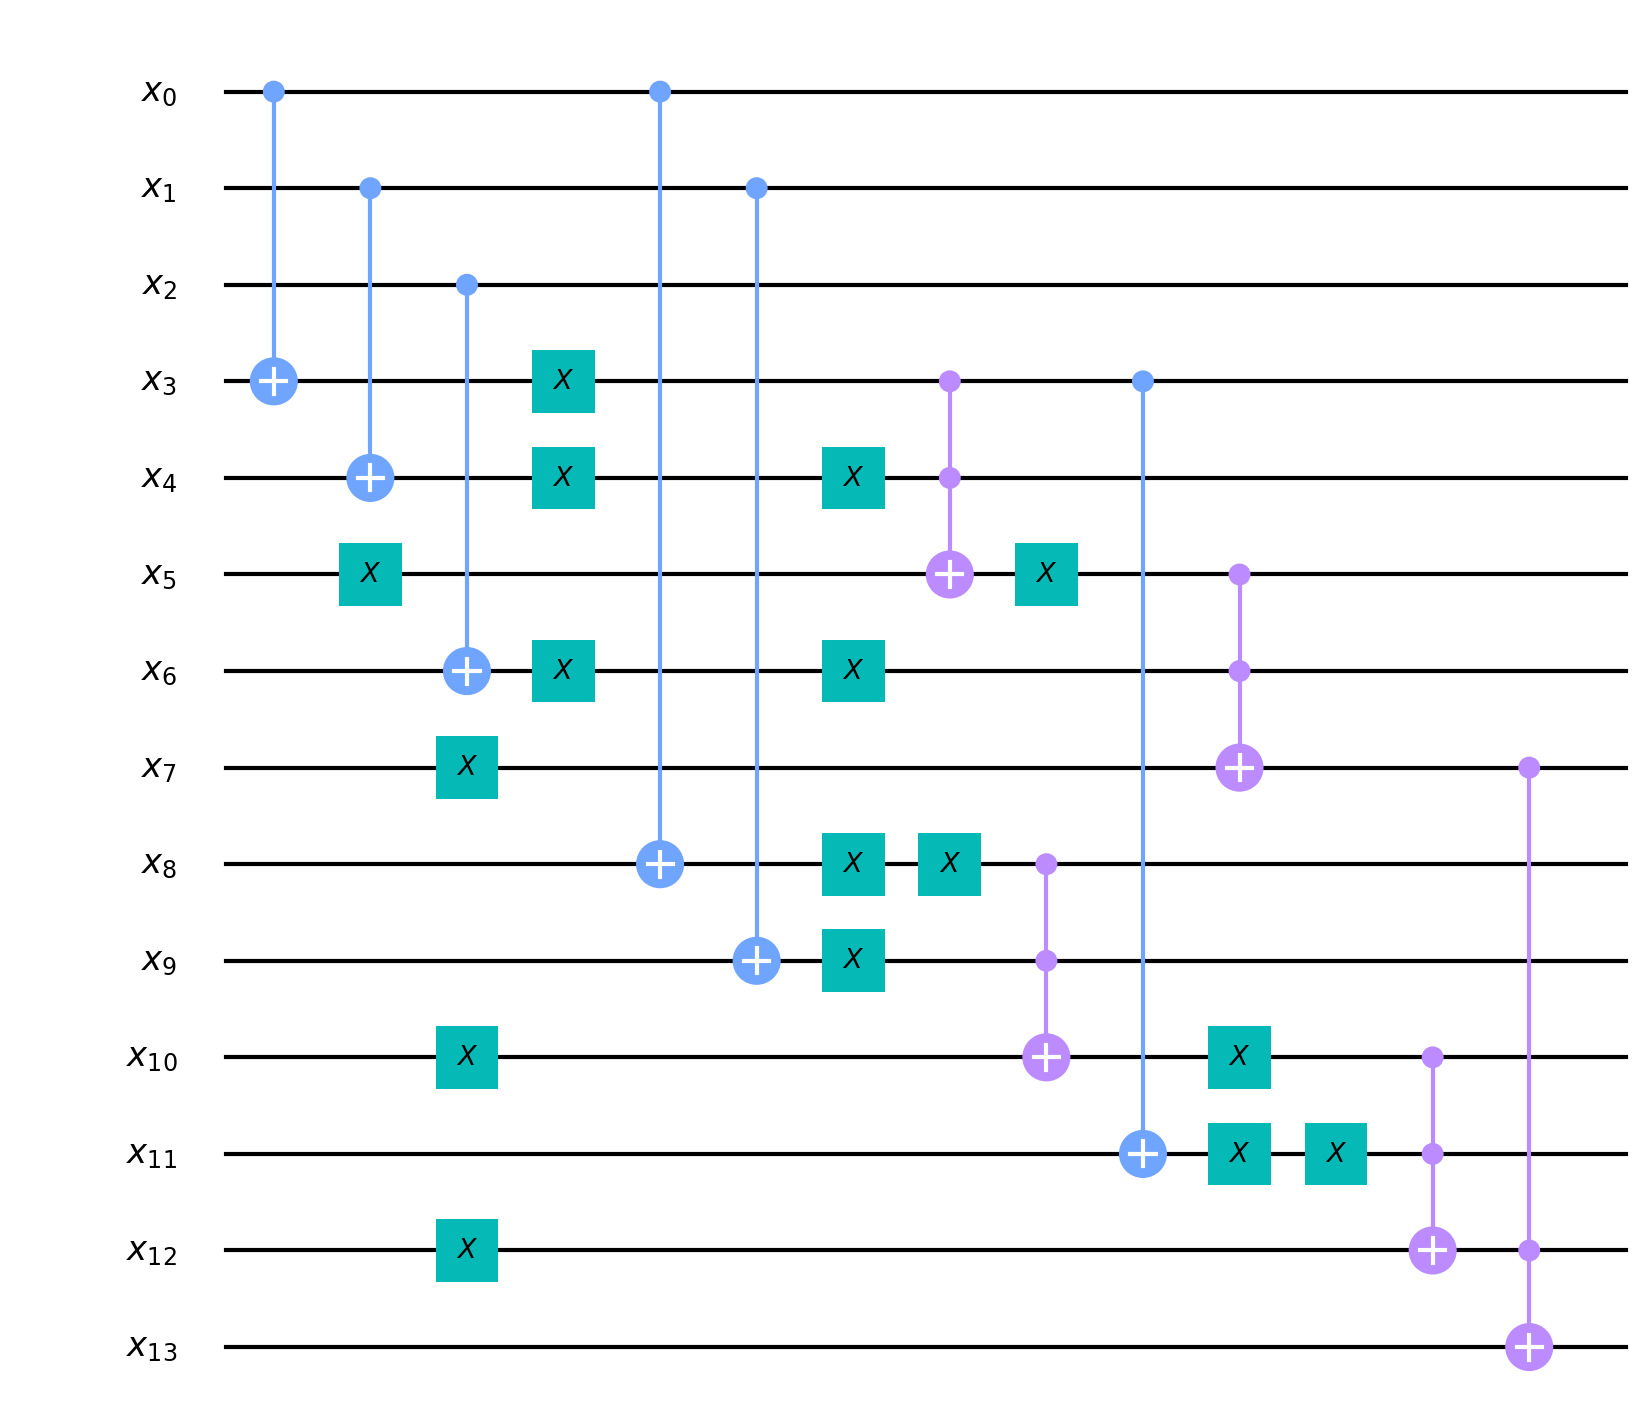
\includegraphics[scale=0.35]{example6.png}
				\caption{CNF circuit}
			\end{figure}
	
			% MEASUREMENT		
				
		\subsection{The Quantum Computer}
		\label{sec:quantumComputer}
			
		\subsection{Grover's Algorithm}
		\label{sec:grover}
		
	\section{Computational Theory}
	\label{sec:computationalTheory}
		
		\subsection{SAT Problem}
		\label{sec:sat}
		
	\section{SAT Implementation}
	\label{sec:satImpl}
		
		\subsection{Classical}
		\label{sec:satClassical}
		
		\subsection{Quantum}
		\label{sec:satQuantum}
		
		\subsection{Classical vs. Quantum}
		\label{sec:satCsatQ}
		
	\section{Conclusions}
	\label{sec:conclusions}
	
	\clearpage
	\begin{appendices}
		\section{Qiskit}
		\label{sec:qiskit}
		
		\section{Code with Qiskit}
		This section contains the list of the snippets of code needed to represent the examples used in the paper. To replicate them consider ti import the following libraries:
		\lstinputlisting[language=python]{code/imports.py}
		
		\label{sec:codeWithQiskit}
			\begin{enumerate}
				\item \label{c:example3} \lstinputlisting[language=python]{code/example3.py}
				
				\item \label{c:example6} \lstinputlisting[language=python]{code/example6.py}
			\end{enumerate}
	\end{appendices}
	
	\clearpage
	\bibliographystyle{plain}
	\nocite{*}
	\bibliography{main.bib}
\end{document}

